A teoria que descreve as interações mediadas por \emph{gluons} é a
QCD\footnote{Sigla em inglês para Cromodinâmica Quântica}. É uma teoria
de calibre não-abeliana, o que significa que os bósons mediadores
de suas interações podem interagir entre si também, formando vértices
constituídos apenas por \emph{gluons}, como na Figura \ref{fourgluon}.

	\usetikzlibrary{trees}
	\usetikzlibrary{decorations.pathmorphing}
	\usetikzlibrary{decorations.markings}
	
	\tikzset{
				    photon/.style={decorate, decoration={snake}, draw=red},
				    electron/.style={draw=blue, postaction={decorate},
				        decoration={markings,mark=at position .55 with {\arrow[draw=blue]{>}}}},
				    gluon/.style={decorate, draw=magenta,
				        decoration={coil,amplitude=4pt, segment length=5pt}} 
				}
				
	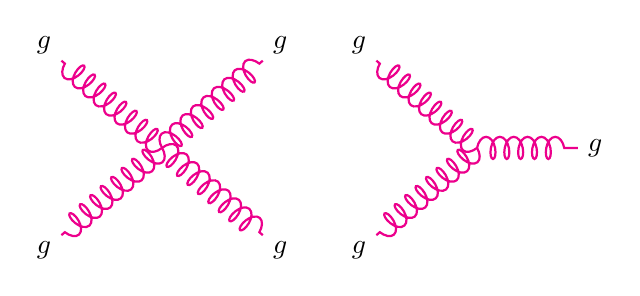
\begin{tikzpicture}[
				        thick,
				        % Set the overall layout of the tree
				        level/.style={level distance=1.5cm},
				        level 2/.style={sibling distance=2.6cm},
				        level 3/.style={sibling distance=2cm}
				    ]
				    \coordinate (4) at (0,0)
				        child[grow=left, level distance=0pt]{
				            child {
				                node {$g$}
				                % The 'edge from parent' is actually not needed because it is
				                % implicitly added.
				                edge from parent [gluon]
				            }
				            child {
				                node {$g$}
				                edge from parent [gluon]
				            }
				        }
				        % I have to insert a dummy child to get the tree to grow
				        % correctly to the right.
				        child[grow=right, level distance=0pt]{
								child {
										node {$g$}
										edge from parent [gluon]
									}
									child {
										node {$g$}
										edge from parent [gluon]
		}
								};

\coordinate (3) at (4,0)
				        child[grow=left, level distance=0pt]{
				            child {
				                node {$g$}
				                % The 'edge from parent' is actually not needed because it is
				                % implicitly added.
				                edge from parent [gluon]
				            }
				            child {
				                node {$g$}
				                edge from parent [gluon]
				            }
				        }
				        % I have to insert a dummy child to get the tree to grow
				        % correctly to the right.
				        child[grow=right, level distance=0pt]{
								child {
										node {$g$}
										edge from parent [gluon]
									}
								};
						\end{tikzpicture}

Uma das consequências desta interação entre os \emph{glons}, é que as linhas
de campo entre um \emph{quark} e um \emph{antiquark} irão estar todas contidas
em uma região aproximadamente cilíndrica entre ambos, como na Figura \ref{linhascampo}.

\begin{figure}[!h]
\centering
 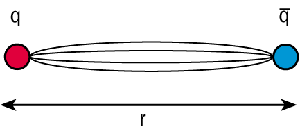
\includegraphics[scale=0.5]{Content/gluonfield.png}
 \caption{Linhas de campo entre um \emph{quark} e um \emph{antiquark}.}
 \label{linhascampo}
\end{figure}

Isso dará origem a uma densidade de energia aproximadamente constante, que dependerá
apenas da distância entre ambos:

\begin{equation}
 V(r) = -\kappa r
\end{equation}

Isso faz com que os \emph{quarks} movam-se sempre sob uma fora constante que muda de direção.
Eventualmente, na região preenchida pelo campo, devido a uma distância grande entre os \emph{quarks},
a energia do campo pode ser grande o suficiente para que um par partícula e anti-partícula se forme.
Quando isso ocorre, a energia fica distribuída em duas regiões devido a efeitos de blindagem, e teremos,
então, dois pares agora independentes, esse processo continua até que todos os pares formados não atingam
mais a distância necessária para a criação de pares. Uma descrição mais detalhada deste processo pode ser
encontrada em \cite{bierlich_rope_2017,andersson_recent_2002,skands_introduction_2013}.